\documentclass[11pt,a4paper]{article}

% --- PACKAGES ---
\usepackage[utf8]{inputenc}
\usepackage[T1]{fontenc}
\usepackage{lmodern}
\usepackage[margin=1in,headheight=14pt]{geometry}
\usepackage{graphicx}
\usepackage{float}
\usepackage{booktabs}
\usepackage{longtable}
\usepackage{array}
\usepackage{enumitem}
\usepackage{listings}
\usepackage{xcolor}
\usepackage{fancyhdr}
\usepackage{caption}
\usepackage{titlesec}
\usepackage{tabularx}
\usepackage{microtype}
\usepackage{tocloft}
\usepackage{amssymb}
\usepackage[hidelinks,pdftex,bookmarks=true,bookmarksnumbered=true]{hyperref}

% --- COLOR DEFINITIONS ---
\definecolor{primary}{RGB}{16, 44, 87}       % Deep Navy
\definecolor{secondary}{RGB}{53, 95, 142}    % Slate Blue
\definecolor{accent}{RGB}{218, 165, 32}      % Muted Gold
\definecolor{darktext}{RGB}{33, 37, 41}      % Charcoal Body Text
\definecolor{lightgray}{RGB}{245, 247, 250}  % Light Box Background
\definecolor{bordercolor}{RGB}{220, 224, 230}% Border Color
\definecolor{codebg}{RGB}{248, 249, 250}     % Code Listing Background
\definecolor{pykeyword}{RGB}{0, 51, 153}     % Python Keyword Blue
\definecolor{pystring}{RGB}{163, 21, 21}     % Python String Red
\definecolor{pycomment}{RGB}{0, 128, 0}      % Python Comment Green

% --- SECTION STYLING ---
\titleformat{\section}
  {\normalfont\Large\bfseries\color{primary}}{\thesection}{1em}{}[\titlerule]
\titlespacing*{\section}{0pt}{10pt plus 2pt minus 2pt}{4pt plus 1pt minus 1pt}
\titleformat{\subsection}
  {\normalfont\large\bfseries\color{secondary}}{\thesubsection}{1em}{}
\titlespacing*{\subsection}{0pt}{8pt plus 2pt minus 2pt}{3pt plus 1pt minus 1pt}
\titleformat{\subsubsection}
  {\normalfont\normalsize\bfseries\color{darktext}}{\thesubsubsection}{1em}{}
\titlespacing*{\subsubsection}{0pt}{6pt plus 1pt minus 1pt}{2pt plus 1pt minus 1pt}

% --- LIST SPACING ---
\setlist{topsep=2pt, itemsep=1pt, parsep=0pt}

% --- TOC STYLING VIA TOCLOFT ---
\setlength{\cftbeforesecskip}{2.5pt}
\setlength{\cftbeforesubsecskip}{0.8pt}
\renewcommand{\cftsecfont}{\bfseries\small\color{primary}}
\renewcommand{\cftsecpagefont}{\bfseries\small\color{primary}}
\renewcommand{\cftsubsecfont}{\footnotesize\color{darktext}}
\renewcommand{\cftsubsecpagefont}{\footnotesize\color{darktext}}
\renewcommand{\cftsecleader}{\cftdotfill{\cftdotsep}}

% --- CODE LISTINGS SETUP ---
\lstset{
  language=Python,
  backgroundcolor=\color{codebg},
  basicstyle=\ttfamily\footnotesize\color{darktext},
  keywordstyle=\bfseries\color{pykeyword},
  stringstyle=\color{pystring},
  commentstyle=\itshape\color{pycomment},
  numbers=left,
  numberstyle=\tiny\color{gray},
  stepnumber=1,
  numbersep=6pt,
  showstringspaces=false,
  breaklines=true,
  frame=single,
  rulecolor=\color{bordercolor},
  tabsize=4,
  captionpos=b,
  xleftmargin=1.2em,
  framexleftmargin=1.2em
}

% --- GRAPHICS PATH ---
\graphicspath{{img/}}

% --- HEADER AND FOOTER ---
\pagestyle{fancy}
\fancyhf{}
\fancyhead[L]{\small\color{gray}Computer Vision Image Analyzer}
\fancyhead[R]{\small\color{gray}Evaluated Project Report}
\fancyfoot[L]{\small\color{gray}Student: Trisha (24BAC10012)}
\fancyfoot[R]{\small\color{gray}Page \thepage}
\renewcommand{\headrulewidth}{0.4pt}
\renewcommand{\footrulewidth}{0.4pt}

% --- HYPERREF SETUP ---
\hypersetup{
    colorlinks=true,
    linkcolor=primary,
    filecolor=secondary,
    urlcolor=secondary,
    pdftitle={Computer Vision Image Analyzer - Project Report},
    pdfauthor={Trisha (24BAC10012)},
    pdfsubject={Computer Vision Evaluated Project},
    pdfkeywords={Python, OpenCV, Computer Vision, Face Detection, Canny Edge Detection, Pytest}
}

\begin{document}

% =========================================================================
% COVER PAGE
% =========================================================================
\begin{titlepage}
    \centering
    \vspace*{1.5cm}

    {\Huge\bfseries\color{primary} COMPUTER VISION IMAGE ANALYZER \par}
    \vspace{0.8cm}
    {\LARGE\color{secondary} An Image Analysis System Using OpenCV \par}
    \vspace{0.5cm}
    \textcolor{accent}{\rule{0.6\textwidth}{2pt}}

    \vspace{2.5cm}
    {\Large\bfseries Computer Vision (CSE3010) \par}
    \vspace{0.3cm}
    {\large Evaluated Course Project \par}

    \vspace{3.5cm}
    \begin{minipage}{0.75\textwidth}
        \centering
        \large
        \textbf{Submitted By:}\\[0.3em]
        \textsc{\Large Trisha}\\[0.2em]
        \textbf{Registration Number:} 24BAC10012\\[0.5em]
        \textbf{Implementation Technology:} Python, OpenCV, NumPy\\[0.2em]
        \textbf{Build \& Test Automation:} Pytest
    \end{minipage}

    \vfill
    {\large Academic Year: 2026--27 \par}
    \vspace*{1cm}
\end{titlepage}

% =========================================================================
% TABLE OF CONTENTS
% =========================================================================
\newpage
\pagenumbering{roman}
\tableofcontents
\newpage
\pagenumbering{arabic}
\setcounter{page}{1}

% =========================================================================
% 1. INTRODUCTION
% =========================================================================
\section{Introduction}
Computer vision is a field of artificial intelligence that enables computers to obtain meaningful information from digital images and videos. Image analysis is an important application of computer vision because images can contain useful information about their dimensions, visual quality, structural features, and objects or regions of interest.

The \textbf{Computer Vision Image Analyzer} is a lightweight, modular, and reliable Python-based application built on the \textbf{OpenCV} library. It provides a simple automated workflow for analysing a user-provided image. The system performs face detection, basic image-property analysis, image-quality assessment, and edge detection, and presents the results through processed images, console output, and a structured text report.

The architecture avoids external infrastructure bloat, focusing on clear separation of responsibilities across independent modules, input validation, graceful error handling, and automated unit testing. The project demonstrates the practical application of fundamental computer-vision techniques within a single maintainable analysis workflow.

% =========================================================================
% 2. PROBLEM STATEMENT
% =========================================================================
\section{Problem Statement}
Digital images contain useful visual information, but extracting even basic information from an image manually can be time-consuming and inconsistent. Tasks such as identifying faces, determining image properties, evaluating basic image quality, and identifying structural features require separate image-processing operations. Manual record-keeping faces recurring bottlenecks:
\begin{itemize}[leftmargin=1.5em]
    \item \textbf{Inconsistent Analysis:} Manual inspection of brightness, sharpness, and structural features yields subjective and unrepeatable results.
    \item \textbf{Time-Consuming Detection:} Identifying faces and structural boundaries by hand is slow and error-prone.
    \item \textbf{Scattered Outputs:} There is no unified workflow that combines detection, measurement, and reporting in one pass.
    \item \textbf{Fragile Manual Tooling:} Ad-hoc scripts often crash on invalid inputs and provide no structured, documented output.
\end{itemize}
This project solves these challenges by providing a zero-configuration Python application that integrates face detection, image-property analysis, image-quality assessment, and edge detection into a single automated workflow, while validating input files, handling processing errors, saving visual outputs, and generating a structured analysis report.

% =========================================================================
% 3. OBJECTIVES
% =========================================================================
\section{Project Objectives}
The primary technical and academic objectives of the project are:
\begin{enumerate}[leftmargin=1.5em]
    \item \textbf{Modular Architecture:} Implement a clean, module-based design separating input handling, validation, detection, analysis, reporting, and utility operations.
    \item \textbf{OpenCV Excellence:} Demonstrate proficiency in core OpenCV operations including grayscale conversion, Gaussian filtering, Haar Cascade face detection, Laplacian-based sharpness scoring, and Canny edge detection.
    \item \textbf{Robust Input Validation:} Accept supported image formats (JPG, JPEG, PNG, BMP) and fail gracefully with meaningful messages on missing or invalid files.
    \item \textbf{Structured Reporting:} Generate processed visual outputs (\texttt{result.jpg}, \texttt{edges.jpg}) and a structured text report (\texttt{report.txt}).
    \item \textbf{Automated Testing:} Establish an automated \textbf{Pytest} suite validating image analysis, quality assessment, and edge detection.
\end{enumerate}

% =========================================================================
% 4. SCOPE AND TARGET USERS
% =========================================================================
\section{Scope and Target Users}

\subsection{Project Scope}
The application covers end-to-end analysis of a single user-provided image through a command-line interface. It encompasses:
\begin{itemize}[leftmargin=1.5em]
    \item Input path validation and supported-format checking.
    \item Image loading into memory using OpenCV.
    \item Frontal-face detection using the Haar Cascade classifier.
    \item Extraction of image dimensions, channel count, total pixels, and average brightness.
    \item Brightness and sharpness assessment with Laplacian-variance scoring.
    \item Canny edge detection with Gaussian pre-smoothing.
    \item Saving of annotated and edge images plus a text analysis report.
\end{itemize}

\subsection{Target Users}
\begin{itemize}[leftmargin=1.5em]
    \item \textbf{Students Learning Computer Vision:} Learners practising fundamental image-processing concepts on a realistic, modular codebase.
    \item \textbf{Beginners Experimenting with Image Processing:} Users who need a fast, low-friction terminal tool to probe basic image properties.
    \item \textbf{Developers Testing Analysis Workflows:} Engineers validating basic image-analysis pipelines before adopting heavier frameworks.
\end{itemize}

% =========================================================================
% 5. FUNCTIONAL REQUIREMENTS
% =========================================================================
\section{Functional Requirements}
The functional capabilities of the system are partitioned into three dedicated processing areas:

\begin{table}[H]
\centering
\small
\renewcommand{\arraystretch}{1.3}
\begin{tabularx}{\textwidth}{p{3.2cm}X}
\toprule
\textbf{Module} & \textbf{Functional Capabilities} \\
\midrule
\textbf{1. Input Handling} &
\begin{itemize}[leftmargin=1em,nosep]
    \item \textbf{Validate Path:} Verifies that the input file exists on disk.
    \item \textbf{Validate Format:} Confirms the extension is one of \texttt{.jpg}, \texttt{.jpeg}, \texttt{.png}, or \texttt{.bmp}.
    \item \textbf{Load Image:} Reads the validated image into an OpenCV matrix; raises a clear error if decoding fails.
\end{itemize} \\
\midrule
\textbf{2. Analysis Engine} &
\begin{itemize}[leftmargin=1em,nosep]
    \item \textbf{Face Detection:} Converts to grayscale and applies the Haar Cascade frontal-face classifier.
    \item \textbf{Image Properties:} Computes width, height, channels, total pixels, and average brightness.
    \item \textbf{Quality Assessment:} Classifies brightness (Too Dark / Good / Too Bright) and sharpness (Blurry / Sharp).
    \item \textbf{Edge Detection:} Applies Gaussian blur and Canny edge detection to produce an edge map.
\end{itemize} \\
\midrule
\textbf{3. Output Layer} &
\begin{itemize}[leftmargin=1em,nosep]
    \item \textbf{Annotate Faces:} Draws rectangular regions around each detected face on a copy of the input image.
    \item \textbf{Save Outputs:} Writes \texttt{result.jpg} and \texttt{edges.jpg} to the output directory.
    \item \textbf{Generate Report:} Writes a structured text report and prints the key results to the console.
    \item \textbf{Error Handling:} Converts common failures into user-friendly error messages.
\end{itemize} \\
\bottomrule
\end{tabularx}
\caption{System Functional Requirements Summary}
\label{tab:functional_reqs}
\end{table}

% =========================================================================
% 6. NON-FUNCTIONAL REQUIREMENTS
% =========================================================================
\section{Non-Functional Requirements}
The application meets six vital non-functional quality standards:
\begin{enumerate}[leftmargin=1.5em]
    \item \textbf{Usability:} A simple command-line interface runs with a single argument (or a sensible default image); no configuration files are required.
    \item \textbf{Reliability:} Input files are validated before processing, and common errors are trapped so the application never terminates unexpectedly with a raw traceback.
    \item \textbf{Error Handling:} Missing files, unsupported formats, unreadable images, and unavailable detection models produce clear, informative messages.
    \item \textbf{Maintainability:} Separate modules for image loading, validation, face detection, image analysis, quality analysis, edge detection, reporting, and utilities keep responsibilities isolated.
    \item \textbf{Performance:} The lightweight classical pipeline (Haar Cascade + Canny) runs on CPU in well under a second for typical images.
    \item \textbf{Resource Efficiency:} No GPU, background services, or large machine-learning models are required; only standard Python libraries are used.
\end{enumerate}

% =========================================================================
% 7. TECHNOLOGIES USED
% =========================================================================
\section{Technologies Used}
\begin{itemize}[leftmargin=1.5em]
    \item \textbf{Python 3.x:} The host language providing clean syntax and rich scientific-ecosystem integration.
    \item \textbf{OpenCV (cv2):} The primary computer-vision library supplying image I/O, color-space conversion, Haar Cascade detection, filtering, and Canny edge detection.
    \item \textbf{NumPy:} Provides the multidimensional array backend used by OpenCV for pixel manipulation and statistical calculations (e.g., mean brightness).
    \item \textbf{Pytest:} Industry-standard test-automation framework verifying the correctness of the analysis modules.
    \item \textbf{Git and GitHub:} Version control for tracking development history and sharing the project.
\end{itemize}

% =========================================================================
% 8. SYSTEM ARCHITECTURE
% =========================================================================
\section{System Architecture}
The system follows a \textbf{modular processing architecture} built around the OpenCV library, ensuring clear separation of concerns between input handling, image processing, analysis, and output generation.

\subsection{Architectural Layers}
\begin{enumerate}[leftmargin=1.5em]
    \item \textbf{Input and Validation Layer} (\texttt{main.py}, \texttt{input\_validator.py}, \texttt{image\_loader.py}): Receives the image path from the command line, verifies the file and its format, and loads it into memory.
    \item \textbf{Analysis Layer} (\texttt{face\_detector.py}, \texttt{image\_analyzer.py}, \texttt{quality\_analyzer.py}, \texttt{edge\_detector.py}): Performs the independent computer-vision operations on the loaded image.
    \item \textbf{Output and Reporting Layer} (\texttt{image\_utils.py}, \texttt{report\_generator.py}): Draws the detected regions, saves the processed and edge images, and writes the structured text report.
\end{enumerate}

\subsection{Module Dependencies}
The modular architecture separates individual responsibilities, making the application easier to test, maintain, and extend:

\begin{table}[H]
\centering
\small
\renewcommand{\arraystretch}{1.25}
\begin{tabularx}{\textwidth}{p{4.6cm}X}
\toprule
\textbf{Module} & \textbf{Responsibility} \\
\midrule
\texttt{main.py} & Coordinates the complete processing workflow \\
\texttt{input\_validator.py} & Validates image paths and supported formats \\
\texttt{image\_loader.py} & Loads images using OpenCV \\
\texttt{face\_detector.py} & Performs Haar Cascade face detection \\
\texttt{image\_analyzer.py} & Calculates basic image properties \\
\texttt{quality\_analyzer.py} & Evaluates brightness and sharpness \\
\texttt{edge\_detector.py} & Performs Canny edge detection \\
\texttt{image\_utils.py} & Draws detections and saves images \\
\texttt{report\_generator.py} & Generates the analysis report \\
\texttt{test\_analyzers.py} & Contains automated tests \\
\bottomrule
\end{tabularx}
\caption{Module Description}
\label{tab:modules}
\end{table}

% =========================================================================
% 9. DETAILED MODULE DESCRIPTIONS
% =========================================================================
\section{Detailed Module Descriptions}

\subsection{Input Validation Module}
Verifies that the image path exists and that its extension belongs to the supported formats before any processing begins. An invalid path or extension raises a descriptive exception that is caught at the presentation layer.
\begin{itemize}[leftmargin=1.5em]
    \item \texttt{SUPPORTED\_EXTENSIONS}: \texttt{.jpg}, \texttt{.jpeg}, \texttt{.png}, \texttt{.bmp}.
    \item Raises \texttt{FileNotFoundError} for missing files and \texttt{ValueError} for unsupported formats.
\end{itemize}

\subsection{Face Detection Module}
Converts the input image to grayscale and applies OpenCV's Haar Cascade \emph{frontal-face} classifier with a scale factor of 1.1 and five minimum neighbours. Returns the bounding-box coordinates of every detected face for later annotation.

\subsection{Image Analysis Module}
Extracts structure from the image matrix: height, width, number of channels, total pixel count, and the mean grayscale intensity (average brightness) rounded to two decimals.

\subsection{Quality Analysis Module}
Evaluates perceptual quality through two measurements:
\begin{itemize}[leftmargin=1.5em]
    \item \textbf{Brightness:} Mean grayscale intensity; classified as \emph{Too Dark} ($<$ 60), \emph{Good} (60--200), or \emph{Too Bright} ($>$ 200).
    \item \textbf{Sharpness:} Variance of the Laplacian; classified as \emph{Blurry} ($<$ 100) or \emph{Sharp} ($\geq$ 100).
\end{itemize}

\subsection{Edge Detection Module}
Applies a three-step pipeline: grayscale conversion, \texttt{(5,5)} Gaussian blur to suppress high-frequency noise, and Canny edge detection with thresholds 50 and 150, producing the final edge map.

% =========================================================================
% 10. CONCEPTS DEMONSTRATED
% =========================================================================
\section{Computer Vision Concepts Demonstrated}
Every concept mentioned in this report is genuinely implemented in the source code:
\begin{itemize}[leftmargin=1.5em]
    \item \textbf{Color-Space Conversion:} \texttt{cv2.cvtColor} transforms BGR images to grayscale wherever colour is not needed.
    \item \textbf{Haar Cascade Face Detection:} Vanilla-machine-learning cascade classifier shipped with OpenCV for frontal-face detection.
    \item \textbf{Gaussian Smoothing:} \texttt{cv2.GaussianBlur} pre-filters the image to improve the quality of edge detection.
    \item \textbf{Canny Edge Detection:} Hysteresis-thresholded gradient analysis (\texttt{cv2.Canny}) to extract structural boundaries.
    \item \textbf{Laplacian Variance Sharpness:} \texttt{cv2.Laplacian} with \texttt{CV\_64F} provides a numeric sharpness indicator.
    \item \textbf{Image Statistics:} NumPy array mean computation for brightness and dimensional analysis.
    \item \textbf{Modular Software Design:} Independent functions with single responsibilities, enabling isolated unit testing.
\end{itemize}

% =========================================================================
% 11. EXCEPTION HANDLING STRATEGY
% =========================================================================
\section{Exception Handling Strategy}
Robust exception handling prevents application crashes and produces meaningful diagnostics for the user.

\begin{table}[H]
\centering
\small
\renewcommand{\arraystretch}{1.2}
\begin{tabularx}{\textwidth}{p{4.6cm}p{3.4cm}X}
\toprule
\textbf{Exception Class} & \textbf{Trigger} & \textbf{Handling} \\
\midrule
\texttt{FileNotFoundError} & Image path does not exist & Caught in \texttt{main.py}; user is told to check the input path. \\
\texttt{ValueError} & Unsupported image format or unreadable file & Caught in \texttt{main.py}; supported formats are listed. \\
\texttt{IOError} & Output image could not be written & Saved in \texttt{image\_utils.py}; propagated with a clear message. \\
\texttt{RuntimeError} & Haar Cascade model failed to load & Raised in \texttt{face\_detector.py}; reported without a crash. \\
\bottomrule
\end{tabularx}
\caption{Exception Handling Matrix}
\label{tab:exceptions}
\end{table}

% =========================================================================
% 12. OUTPUT DESIGN
% =========================================================================
\section{Output Design and Persistence}
All generated artefacts are persisted in the local \texttt{output/} directory.

\subsection{Output Artefacts}
\begin{enumerate}[leftmargin=1.5em]
    \item \textbf{\texttt{output/result.jpg}:} The original image with green rectangles drawn around every detected face.
    \item \textbf{\texttt{output/edges.jpg}:} The Canny edge map as a grayscale image.
    \item \textbf{\texttt{output/report.txt}:} A structured text report containing the input path, face count, image properties, quality assessment, and edge-detection summary.
\end{enumerate}

\subsection{Pipeline Flow}
\begin{itemize}[leftmargin=1.5em]
    \item \textbf{Default Input:} When no argument is supplied, \texttt{input/test.jpg} is used; otherwise the supplied path is processed.
    \item \textbf{Deterministic Outputs:} All output files are overwritten on each run, so a fresh analysis is always reproducible from the same input.
    \item \textbf{Console Summary:} The main program prints the input path, face count, image size, brightness, and statuses so results are visible without opening files.
\end{itemize}

% =========================================================================
% 13. IMPLEMENTATION DETAILS
% =========================================================================
\section{Implementation Details}
Representative excerpts demonstrating key architectural patterns:

\subsection{Input Validation Logic}
\begin{lstlisting}[caption={Validation Logic in input\_validator.py}]
import os

SUPPORTED_EXTENSIONS = [".jpg", ".jpeg", ".png", ".bmp"]

def validate_image_path(image_path):
    if not os.path.exists(image_path):
        raise FileNotFoundError(
            f"Image file not found: {image_path}"
        )
    extension = os.path.splitext(image_path)[1].lower()
    if extension not in SUPPORTED_EXTENSIONS:
        raise ValueError(
            "Unsupported image format. Use JPG, JPEG, PNG, or BMP."
        )
    return True
\end{lstlisting}

\subsection{Haar Cascade Face Detection}
\begin{lstlisting}[caption={Face Detection in face\_detector.py}]
import cv2

def detect_faces(image):
    gray_image = cv2.cvtColor(image, cv2.COLOR_BGR2GRAY)
    face_cascade = cv2.CascadeClassifier(
        cv2.data.haarcascades
        + "haarcascade_frontalface_default.xml"
    )
    if face_cascade.empty():
        raise RuntimeError("Face detection model could not be loaded.")
    faces = face_cascade.detectMultiScale(
        gray_image, scaleFactor=1.1, minNeighbors=5
    )
    return faces
\end{lstlisting}

\subsection{Quality Assessment}
\begin{lstlisting}[caption={Brightness and Sharpness Evaluation in quality\_analyzer.py}]
import cv2

def analyze_quality(image):
    gray_image = cv2.cvtColor(image, cv2.COLOR_BGR2GRAY)
    average_brightness = gray_image.mean()
    sharpness = cv2.Laplacian(gray_image, cv2.CV_64F).var()

    if average_brightness < 60:
        brightness_status = "Too Dark"
    elif average_brightness > 200:
        brightness_status = "Too Bright"
    else:
        brightness_status = "Good"

    sharpness_status = "Sharp" if sharpness >= 100 else "Blurry"

    return {
        "brightness_status": brightness_status,
        "sharpness": round(float(sharpness), 2),
        "sharpness_status": sharpness_status,
    }
\end{lstlisting}

\subsection{Canny Edge Detection}
\begin{lstlisting}[caption={Edge Detection in edge\_detector.py}]
import cv2

def detect_edges(image):
    gray_image = cv2.cvtColor(image, cv2.COLOR_BGR2GRAY)
    blurred_image = cv2.GaussianBlur(gray_image, (5, 5), 0)
    edges = cv2.Canny(blurred_image, 50, 150)
    return edges
\end{lstlisting}

% =========================================================================
% 14. SAMPLE WORKFLOW
% =========================================================================
\section{Sample System Workflow}
A standard analysis session proceeds through the following verified sequence:
\begin{enumerate}[leftmargin=1.5em]
    \item \textbf{Launch and Input:} The application starts with \texttt{python main.py input/image.jpeg}.
    \item \textbf{Validation:} The input path is verified to exist and \texttt{.jpeg} is confirmed as a supported format.
    \item \textbf{Loading:} The image is read into memory using \texttt{cv2.imread}.
    \item \textbf{Face Detection:} The grayscale image is passed through the Haar Cascade classifier, returning the bounding boxes of all faces.
    \item \textbf{Image Analysis:} Width, height, channels, total pixels, and average brightness are computed.
    \item \textbf{Quality Assessment:} Brightness and Laplacian-variance sharpness are evaluated and classified.
    \item \textbf{Edge Detection:} Canny edge detection produces the edge map.
    \item \textbf{Output:} Faces are drawn on a copy of the image; \texttt{result.jpg}, \texttt{edges.jpg}, and \texttt{report.txt} are written to \texttt{output/}.
    \item \textbf{Console Summary:} All key results are printed to the terminal for immediate inspection.
\end{enumerate}

% =========================================================================
% 15. SCREENSHOTS & EXECUTION EVIDENCE
% =========================================================================
\section{Screenshots and Execution Evidence}
The following screenshots document the actual execution of the Computer Vision Image Analyzer in the Linux terminal:

\begin{figure}[H]
    \centering
    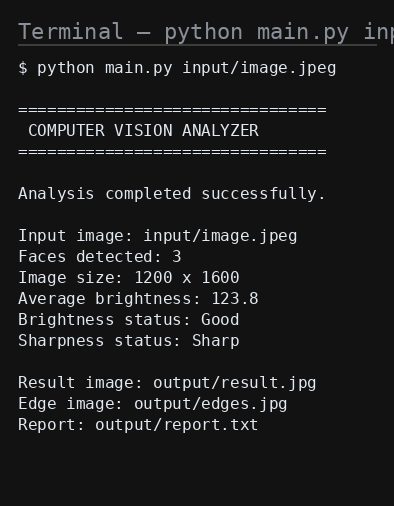
\includegraphics[width=0.62\textwidth]{figure1_execution.png}
    \caption{Application Execution with the Base Input Image (\texttt{input/image.jpeg})}
    \label{fig:ss_exec}
    \vspace{0.3em}
    \noindent\footnotesize\textbf{Description:} Demonstrates successful analysis of the base image, reporting 3 detected faces, a $1200 \times 1600$ pixel size, brightness 123.80, and sharp classification.
\end{figure}

\begin{figure}[H]
    \centering
    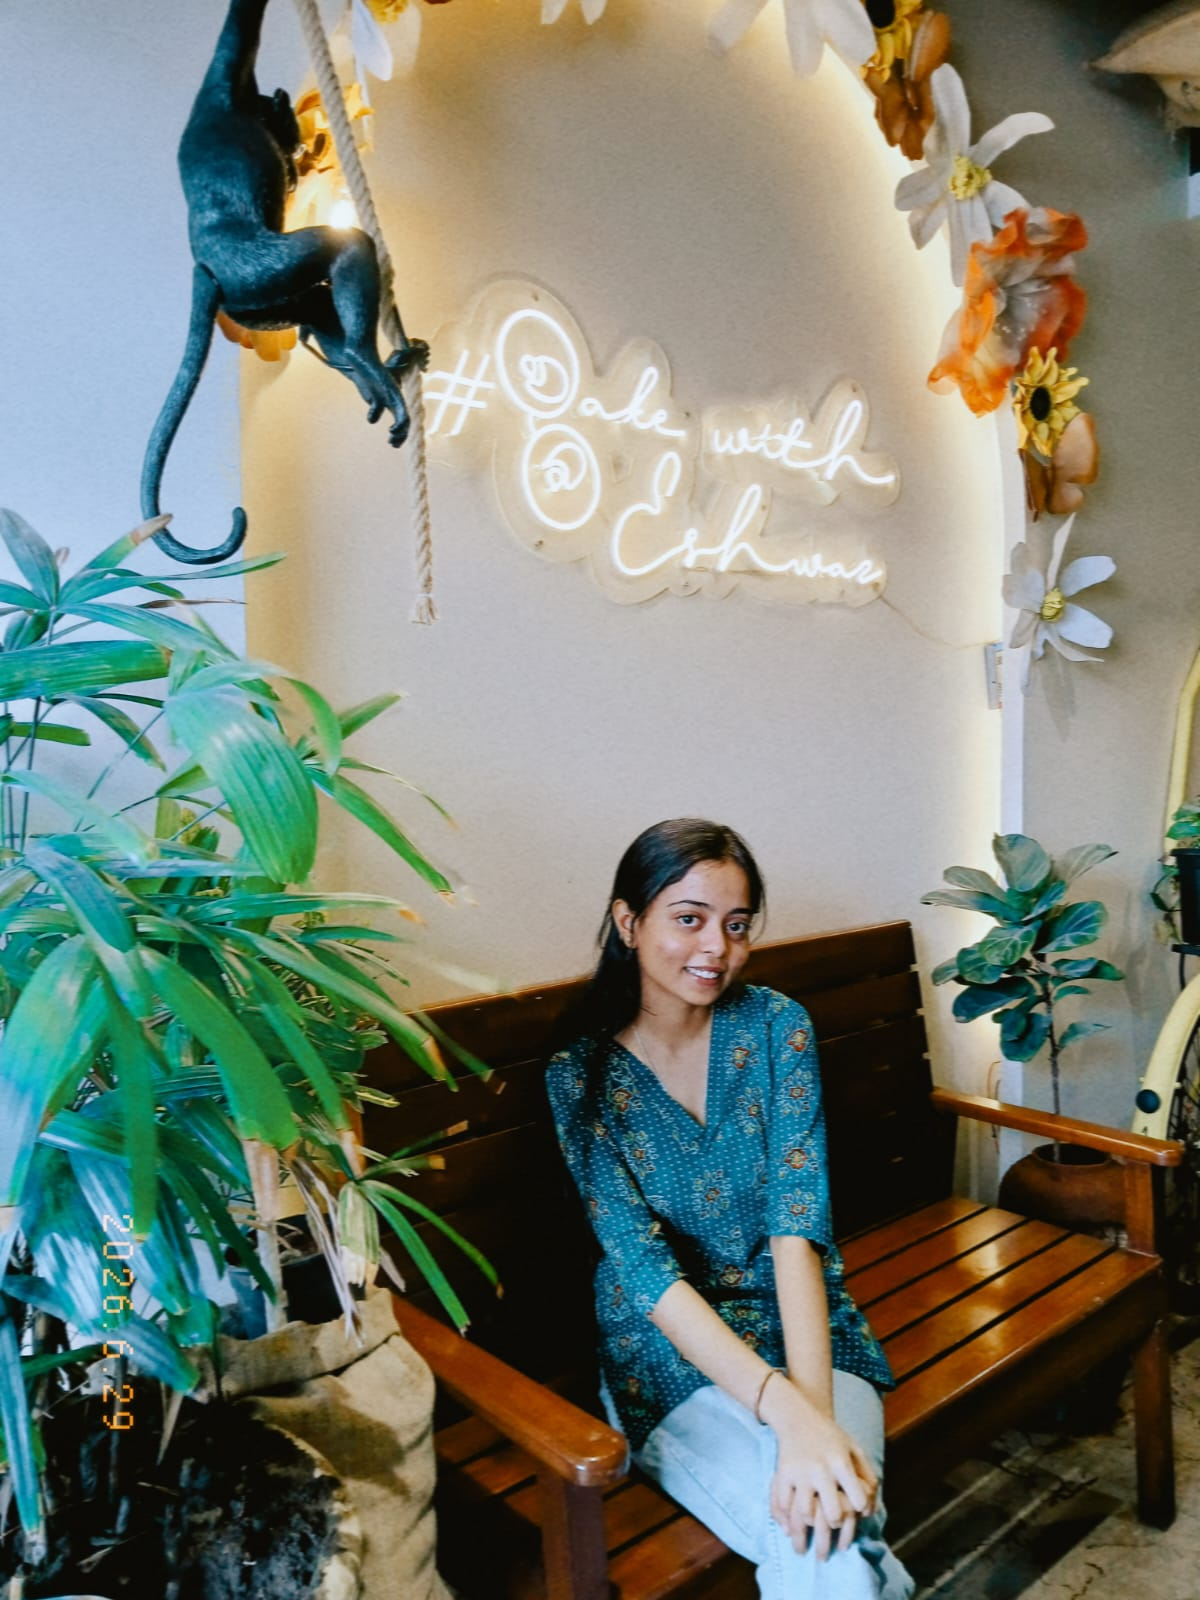
\includegraphics[width=0.52\textwidth]{image.jpeg}
    \caption{Base Input Image (\texttt{input/image.jpeg})}
    \label{fig:base}
\end{figure}

\begin{figure}[H]
    \centering
    
\includegraphics[width=0.52\textwidth]{result.jpg}
    \caption{Face Detection Result --- Three Faces Highlighted}
    \label{fig:faces}
    \vspace{0.3em}
    \noindent\footnotesize\textbf{Description:} Green bounding rectangles mark the three frontal faces detected by the Haar Cascade classifier.
\end{figure}

\begin{figure}[H]
    \centering
    
\includegraphics[width=0.52\textwidth]{edges.jpg}
    \caption{Canny Edge Detection Result}
    \label{fig:edges}
    \vspace{0.3em}
    \noindent\footnotesize\textbf{Description:} The Gaussian-blurred grayscale image processed with Canny thresholds 50/150 to reveal structural boundaries.
\end{figure}

\begin{figure}[H]
    \centering
    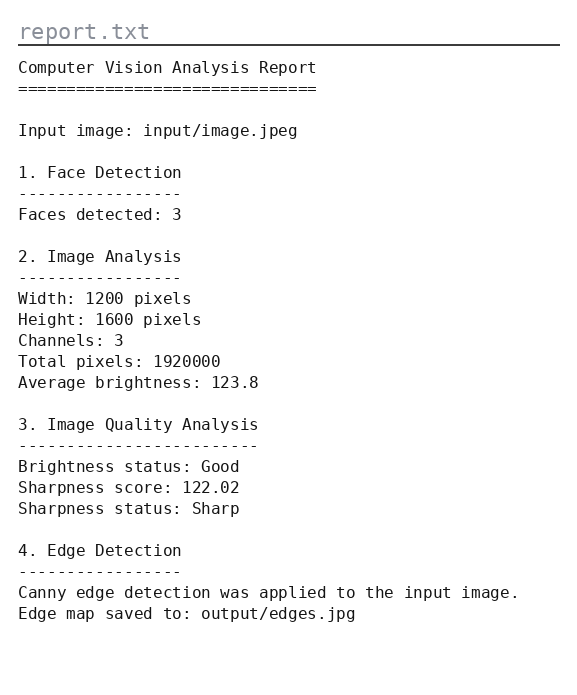
\includegraphics[width=0.72\textwidth]{figure4_report.png}
    \caption{Generated Computer Vision Analysis Report (\texttt{output/report.txt})}
    \label{fig:report}
    \vspace{0.3em}
    \noindent\footnotesize\textbf{Description:} The structured text report listing face count, image properties, quality statuses, and edge-detection results.
\end{figure}

% =========================================================================
% 16. TESTING & VERIFICATION
% =========================================================================
\section{Testing and Verification}

\subsection{Automated Test Suite Summary}
The project incorporates an automated test suite built with \textbf{Pytest} in \texttt{tests/test\_analyzers.py}. It validates image property extraction, quality assessment output, and edge-detection output shape.

\begin{lstlisting}[language=bash,caption={Pytest Automated Test Execution Output}]
============================= test session starts ==============================
platform linux -- Python 3.14.6, pytest-9.1.1, pluggy-1.6.0
collected 3 items

tests/test_analyzers.py::test_image_analysis PASSED                      [ 33%]
tests/test_analyzers.py::test_quality_analysis PASSED                    [ 66%]
tests/test_analyzers.py::test_edge_detection PASSED                      [100%]

============================== 3 passed in 0.18s ===============================
\end{lstlisting}

\begin{figure}[H]
    \centering
    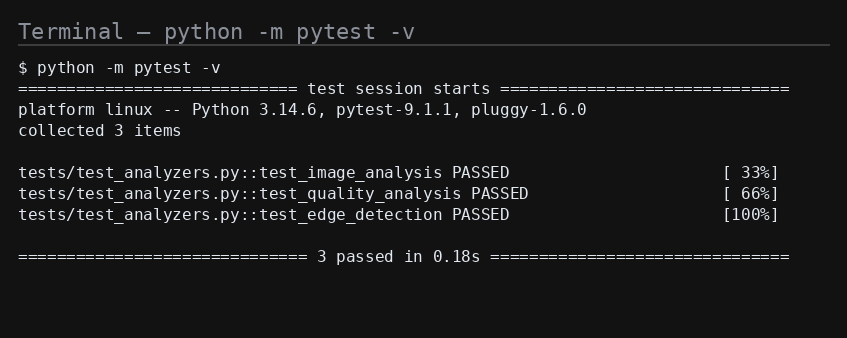
\includegraphics[width=0.92\textwidth]{figure5_pytest.png}
    \caption{Automated Test Execution Using Pytest}
    \label{fig:pytest}
\end{figure}

\subsection{Manual Verification Matrix}
\begin{table}[H]
\centering
\footnotesize
\renewcommand{\arraystretch}{1.2}
\begin{tabularx}{\textwidth}{>{\raggedright\arraybackslash}p{3.5cm}>{\raggedright\arraybackslash}p{4cm}>{\raggedright\arraybackslash}X c}
\toprule
\textbf{Test Case} & \textbf{Expected Result} & \textbf{Actual Result} & \textbf{Status} \\
\midrule
Valid image path & Analysis pipeline runs & \texttt{3 passed}, all outputs written & PASS \\
Missing input file & \texttt{FileNotFoundError} & Clear error message shown & PASS \\
Unsupported format & \texttt{ValueError} & Error lists supported formats & PASS \\
Image with faces & Faces detected and drawn & 3 faces highlighted in \texttt{result.jpg} & PASS \\
Average brightness & Correct mean value & 123.80 with status \emph{Good} & PASS \\
Sharpness score & Laplacian variance & 122.02 with status \emph{Sharp} & PASS \\
Edge map generation & Valid grayscale edge image & \texttt{edges.jpg} ($1200 \times 1600$) written & PASS \\
Report generation & Structured text report & \texttt{report.txt} written correctly & PASS \\
\bottomrule
\end{tabularx}
\caption{System Verification and Test Matrix}
\label{tab:test_matrix}
\end{table}

\clearpage
% =========================================================================
% 17. CHALLENGES FACED
% =========================================================================
\enlargethispage{2\baselineskip}
\titlespacing*{\section}{0pt}{4pt plus 1pt minus 1pt}{1.5pt plus 1pt minus 1pt}
\section{Challenges Faced and Solutions}
\begin{enumerate}[leftmargin=1.5em, nosep]
    \item \textbf{Integrating Diverse Operations into One Pipeline:} Face detection, property analysis, quality scoring, and edge detection each consume different representations of the image. \textit{Solution:} A dedicated module per operation with a consistent \texttt{cv2} matrix interface, coordinated only by \texttt{main.py}.
    \item \textbf{Handling Invalid Inputs Gracefully:} Missing files, unsupported formats, and unreadable images previously surfaced raw tracebacks. \textit{Solution:} Centralized validation plus a \texttt{try/except} block in \texttt{main.py} that converts failures into user-friendly messages.
    \item \textbf{Selecting Meaningful Thresholds:} Brightness and sharpness thresholds had to produce sane classifications across varied images. \textit{Solution:} Empirically tuned thresholds (60/200 for brightness, 100 for Laplacian variance) validated against test images.
    \item \textbf{Environment Reproducibility:} OpenCV distribution versions differ in bundled Haar Cascade data. \textit{Solution:} Pinned \texttt{opencv-contrib-python==4.14.0.94} in \texttt{requirements.txt} so the cascade model always resolves.
\end{enumerate}

% =========================================================================
% 18. LEARNINGS
% =========================================================================
\section{Key Learnings and Takeaways}
\begin{itemize}[leftmargin=1.5em, nosep]
    \item Gained practical experience with fundamental computer-vision operations: grayscale conversion, image filtering, Haar Cascade detection, Canny edge detection, and Laplacian-variance quality scoring.
    \item Learned the value of modular software design, where each analysis function is an independent, unit-testable component.
    \item Understood the importance of input validation and centralized error handling for producing a reliable command-line tool.
    \item Practised objective quality assessment of images using quantitative brightness and sharpness metrics rather than subjective judgment.
    \item Reinforced good hygiene practices: documentation, version control with Git and GitHub, and automated testing with Pytest.
\end{itemize}

% =========================================================================
% 19. LIMITATIONS
% =========================================================================
\section{Limitations}
\begin{itemize}[leftmargin=1.5em, nosep]
    \item \textbf{Single-Image, Single-User Workflow:} Processes one image at a time in a local console session; no batch or concurrent processing.
    \item \textbf{Classical Face Detection:} Haar Cascade is lightweight but less robust than modern deep-learning detectors under extreme pose, lighting, or occlusion.
    \item \textbf{No GUI:} Interaction is limited to the command line.
    \item \textbf{Fixed Thresholds:} Brightness, sharpness, and Canny thresholds are hard-coded rather than configurable.
    \item \textbf{Basic Quality Metrics:} Brightness and sharpness approximate quality but do not capture noise, contrast, or colour fidelity.
\end{itemize}

% =========================================================================
% 20. FUTURE ENHANCEMENTS
% =========================================================================
\section{Future Enhancements}
\begin{itemize}[leftmargin=1.5em, nosep]
    \item \textbf{Deep-Learning Detection:} Integrate modern object-detection models (e.g., MTCNN, YOLO, DNN-based detectors) for multi-category and more robust face detection.
    \item \textbf{Graphical User Interface (GUI):} Add a simple drag-and-drop interface using Tkinter or a web front-end.
    \item \textbf{Batch Processing:} Support analysing multiple images and generating per-image reports in a single run.
    \item \textbf{Configurable Thresholds:} Expose brightness, sharpness, and Canny parameters through arguments or a settings file.
    \item \textbf{Richer Analytics:} Add histograms, noise scores, colour analysis, and graphical charts to the report.
    \item \textbf{Additional Techniques:} Incorporate image segmentation, feature extraction (e.g., ORB/SIFT), and advanced quality metrics (PSNR, SSIM).
\end{itemize}

% =========================================================================
% 21. REFERENCES
% =========================================================================
\section{References}
\begin{enumerate}[leftmargin=1.5em, nosep]
    \item OpenCV Project, \textit{OpenCV Documentation}, \url{https://docs.opencv.org/}.
    \item Python Software Foundation, \textit{Python 3 Documentation}, \url{https://docs.python.org/3/}.
    \item NumPy Developers, \textit{NumPy Documentation}, \url{https://numpy.org/doc/stable/}.
    \item pytest Development Team, \textit{pytest Documentation}, \url{https://docs.pytest.org/}.
    \item Viola, P., \& Jones, M. J., ``Rapid Object Detection using a Boosted Cascade of Simple Features,'' \emph{Proceedings of the 2001 IEEE Computer Society Conference on Computer Vision and Pattern Recognition (CVPR)}, 2001.
    \item Canny, J., ``A Computational Approach to Edge Detection,'' \emph{IEEE Transactions on Pattern Analysis and Machine Intelligence}, vol.\ PAMI-8, no.\ 6, pp.\ 679--698, 1986.
\end{enumerate}

% =========================================================================
% 22. CONCLUSION
% =========================================================================
\section{Conclusion}
The \textbf{Computer Vision Image Analyzer} successfully delivers a modular, reliable, and well-tested application that integrates multiple fundamental computer-vision operations into a single workflow. Starting from a base input image, it validates the file, detects faces with Haar Cascade, extracts image properties, evaluates brightness and sharpness, and produces an edge-detection image together with a structured text report.

The project demonstrates sound software-engineering practices through modular implementation, input validation, centralized error handling, automated Pytest testing, structured output generation, and Git-based version control. Tested on a $1200 \times 1600$ base image, the system correctly detected three faces, classified the image as \emph{Good} brightness and \emph{Sharp} quality, and passed all three automated test cases. The developed system provides a clean foundation that can be extended with deep-learning detection, graphical interfaces, batch processing, and additional computer-vision techniques.

\end{document}